% !TEX TS-program = lualatex
% !TEX encoding = UTF-8 Unicode

\documentclass[12pt, letterpaper]{article}

%%BIBLIOGRAPHY- This uses biber/biblatex to generate bibliographies according to the
%%Unified Style Sheet for Linguistics
\usepackage[main=american, german]{babel}% Recommended
\usepackage{csquotes}% Recommended
\usepackage[backend=biber,
        style=unified,
        maxcitenames=3,
        maxbibnames=99,
        natbib,
        url=false]{biblatex}
\addbibresource{Dissertation.bib}
\setcounter{biburlnumpenalty}{100}  % allow URL breaks at numbers
% \setcounter{biburlucpenalty}{100}   % allow URL breaks at uppercase letters
% \setcounter{biburllcpenalty}{100}   % allow URL breaks at lowercase letters

%%TYPOLOGY
\usepackage[svgnames]{xcolor} % Specify colors by their 'svgnames', for a full list of all colors available see here: http://www.latextemplates.com/svgnames-colors
%\usepackage[compact]{titlesec}
%\titleformat{\section}[runin]{\normalfont\bfseries}{\thesection.}{.5em}{}[.]
%\titleformat{\subsection}[runin]{\normalfont\scshape}{\thesubsection}{.5em}{}[.]
\usepackage[hmargin=1in,vmargin=1in]{geometry}  %Margins          
\usepackage{graphicx}	%Inserting graphics, pictures, images 		
\usepackage{stackengine} %Package to allow text above or below other text, Also helpful for HG weights 
\usepackage{fontspec} %Selection of fonts must be ran in XeLaTeX or LuaLateX
\usepackage{amssymb} %Math symbols
\usepackage{amsmath} % Mathematical enhancements for LaTeX
\usepackage{setspace} %Linespacing
\usepackage{multicol} %Multicolumn text
\usepackage{enumitem} %Allows for continuous numbering of lists over examples, etc.
\usepackage{multirow} %Useful for combining cells in tablesbrew 
\usepackage{booktabs}
\usepackage{hanging}
\usepackage{fancyhdr} %Allows for the 
\pagestyle{fancy}
\fancyhead[L]{\textit{Draft}} 
\fancyhead[R]{\textit{\today}} 
\fancyfoot[L,R]{} 
\fancyfoot[C]{\thepage} 
\renewcommand{\headrulewidth}{0.4pt}
\setlength{\headheight}{14.5pt} % ...at least 14.49998pt
% \usepackage{fourier} % This allows for the use of certain wingdings like bombs, frowns, etc.
% \usepackage{fourier-orns} %More useful symbols like bombs and jolly-roger, mostly for OT
\usepackage[colorlinks,allcolors={black},urlcolor={blue}]{hyperref} %allows for hyperlinks and pdf bookmarks
% \usepackage{url} %allows for urls
% \def\UrlBreaks{\do\/\do-} %allows for urls to be broken up
\usepackage[normalem]{ulem} %strike out text. Handy for syntax
\usepackage{datetime2}
\usepackage{tcolorbox}
\usepackage{todonotes} % Creates todo marginalia
\usepackage{lineno}\linenumbers 

%%FONTS
\setmainfont{Libertinus Serif}
% \setmainfont{Times New Roman}
\setsansfont{Libertinus Sans}
\setmonofont[Scale=MatchLowercase]{Libertinus Mono}
\newfontfamily\ipa{Doulos SIL}

%%PACKAGES FOR LINGUISTICS
%\usepackage{OTtablx} %Generating tableaux with using TIPA
% \usepackage[noipa]{OTtablx} % Use this one generating tableaux without using TIPA
%\usepackage[notipa]{ot-tableau} % Another tableau drawing packing use for posters.
\usepackage{linguex} % Linguistic examples
% \usepackage{langsci-linguex} % Linguistic examples
% \usepackage{langsci-gb4e} % Language Science Press' modification of gb4e
% \usepackage{langsci-avm} % Language Science Press' AVM package
\usepackage{tikz} % Drawing Hasse diagrams
% \usepackage{pst-asr} % Drawing autosegmental features
\usepackage{pstricks} % required for pst-asr, OTtablx, pst-jtree.
% \usepackage{pst-jtree} 	% Syntax tree draawing software
% \usepackage{tikz-qtree}	% Another syntax tree drawing software. Uses bracket notation.
\usepackage[linguistics]{forest}	% Another syntax tree drawing software. Uses bracket notation.
% \usepackage{ling-macros} % Various linguistic macros. Does not work with linguex.
% \usepackage{covington} % Another linguistic examples package.
\usepackage{leipzig} %	Offers support for Leipzig Glossing Rules

%%LEIPZIG GLOSSING FOR ZAPOTEC
\newleipzig{el}{el}{elder} % Elder pronouns
\newleipzig{hu}{hu}{human} % Human pronouns
\newleipzig{an}{an}{animate} % Animate pronouns
\newleipzig{in}{in}{inanimate} % Inanimate pronouns
\newleipzig{pot}{pot}{potential} % Potential Aspect
\newleipzig{cont}{cont}{continuative} % Continuative Aspect
\newleipzig{stat}{stat}{stative} % Stative Aspect
\newleipzig{and}{and}{andative} % Andative Aspect
\newleipzig{ven}{ven}{venative} % Venative Aspect
% \newleipzig{res}{res}{restitutive} % Restitutive Aspect
\newleipzig{rep}{rep}{repetitive} % Repetitive Aspect

%%TITLE INFORMATION
\title{TITLE}
\author{Mykel Loren Brinkerhoff}
\date{\today}

%%MACROS
\newcommand{\sub}[1]{\textsubscript{#1}}
\newcommand{\supr}[1]{\textsuperscript{#1}}
\providecommand{\lsptoprule}{\midrule\toprule}
\providecommand{\lspbottomrule}{\bottomrule\midrule}
\newcommand{\fittable}[1]{\resizebox{\textwidth}{!}{#1}}

\makeatletter
\renewcommand{\paragraph}{%
  \@startsection{paragraph}{4}%
  {\z@}{0ex \@plus 1ex \@minus .2ex}{-1em}%
  {\normalfont\normalsize\bfseries}%
}
\makeatother
\parindent=10pt


\begin{document}

%%If using linguex, need the following commands to get correct LSA style spacing
%% these have to be after  \begin{document}
    % \setlength{\Extopsep}{6pt}
    % \setlength{\Exlabelsep}{9pt}		%effect of 0.4in indent from left text edge
%%

%% Line spacing setting. Comment out the line spacing you do not need. Comment out all if you want single spacing.
%	\doublespacing
	\onehalfspacing

\begin{center}
     {\Large \textbf{On Residual H1* as a measure of voice quality}}
     \vspace{6pt}

     Mykel Loren Brinkerhoff \& Grant McGuire
\end{center}
%\maketitle
%\maketitleinst
\thispagestyle{fancy}

% \tableofcontents

\begin{abstract}
    text.
    \\
    Keywords:
\end{abstract}

%------------------------------------
\section{Introduction} \label{sec:Introduction}
%------------------------------------


%------------------------------------
\section{Santiago Laxopa Zapotec} \label{sec:SLZ}
%------------------------------------

Santiago Laxopa Zapotec is a Northern Zapotec language of Oto-manguean language family \citep{adlerAcousticsPhonationTypes2016,adlerDerivationVerbInitiality2018,foleyForbiddenCliticClusters2018,foleyExtendingPersonCaseConstraint2020,sichelPronounsAttractionSierra2020,
sichelFeaturalLifeNominals2020,brinkerhoffDownstepSantiagoLaxopaMFM,brinkerhoffTonalPatternsTheir2022}. It is spoken by 981 people in the municipality of Santiago Laxopa, Ixtlán, Oaxaca, Mexico \citep{SantiagoLaxopaEconomy} and a small number of other speakers in diaspora throughout Mexico and the United States. Similar to other Oto-manguean languages, Santiago Laxopa Zapotec is laryngeally complex. According to \citet{silvermanLaryngealComplexityOtomanguean1997,silvermanPhasingRecoverability1997,blankenshipTimeCourseBreathiness1997,blankenshipTimingNonmodalPhonation2002}, laryngeal complexity refers to how these languages make use of both contrastive tone and contrastive voice quality. 

Santiago Laxopa Zapotec exhibits the standard five vowel inventory, which are further distinghuished by the use of a four-way contrast in voice quality. This variety is unique for being a Northern Core Zapotec that has developed breathy
voice in addition to the two types of laryngealization that characterize the rest of the
Zapotec languages, namely checked and rearticulated (see \cite{ariza-garciaPhonationTypesTones2018} for a typological study of voice quality distinctions in Zapotec languages). This contrast can be seen in the four-way near-minimal quadruple in \ref{ex:Contrast}.

\ex. Four-way near-minimal contrast for voice quality in Santiago Laxopa Zapotec. \label{ex:Contrast}
  \a. Modal voice\\
  \textit{ya} [ {\ipa ʝa˦} ] ‘temazcal’
  \b. Breathy voice\\ 
  \textit{yah} [ {\ipa ʝa̤˨} ] ‘iron’
  \c. Checked \\
  \textit{cha’} [ {\ipa t͡ʃaa̰˨} ] ‘pot’
  \d. Rearticulated\\ 
  \textit{ya’a} [ {\ipa ʝaa̰a˨} ] ‘market’
  \z. 
\z. 

Additionally, being an Oto-manguean language, Santiago Laxopa Zapotec is tonal with three level tones (H, M, and L) and two contours (MH and HL) that are allowed to appear on nouns \citep{brinkerhoffTonalPatternsTheir2022}.  

These contrasts in voice quality present a rich array of information for testing the reliability of the voice quality measures. 

%------------------------------------
\section{Methodology} \label{sec:Methods}
%------------------------------------

%------------------------------------
\subsection{Elicitation} \label{sec:Elicitation}
%------------------------------------
Ten native speakers of SLZ (five female; five male) participated in a wordlist eliciation. Elication was done in the pueblo of Santiago Laxopa, Ixtlán, Oaxaca, Mexcio during the summer of 2022 on a Zoom H4n handheld recorder (16 bit, 44.5 Khz). 

The wordlist consisted of 72 items repeated three times each in isolation and the carrier sentence \textit{Shnia' X chonhe lhas} ``I say X three times''.\footnote{See Appendix 1 for wordlist} Between these 76 words, there were 11 words with breathy voice, 9 with rearticulated, 10 with checked voice, and 42 with modal. Thirteen of the 76 words were disyllabic and the majority contained the same phonation type. Of those thirteen only five words contained mixed voicing.

%------------------------------------
\subsection{Data Processing} \label{sec:Processing}
%------------------------------------

Each vowel from the target words in the carrier sentence condition was labeled following \citet{garellekAcousticDiscriminabilityComplex2020} for where the vowel began and ended. Each vowel from the word list was annotated for speaker, word, vowel, tone, voice quality, and utterance number. This labeling was conducted for each of the vowels located in the target word from the elicitation list from the carrier sentences.

These vowels were then extracted and fed into VoiceSauce for acoustic measuring \citep{shueVOICESAUCEProgramVoice2009}. Formants were measured using the Snack \citep{sjolanderSnackSoundToolkit2004} while the fundamental frequency (\textit{f0}) was measured using the STRAIGHT algorithm \citep{kawaharaInstantaneousfrequencybasedPitchExtraction1998}. Spectral slope measures were corrected for formants and bandwidths \citep{hansonGlottalCharacteristicsFemale1997,iseliAgeSexVowel2007}. Each vowel was measured with ten equal time intervals, resulting in 22890 data points in total.

The data was cleaned of outliers following the same steps taken by \citet{chaiH1H2Acoustic2022} in their study. The H1*, H1*–H2*, and H1*-A3 and \textit{f0} values were z-scored by speaker to reduce the variation between speakers and provide a way to directly compare the different measures on the same scale. Data points with an absolute z-score value larger than 3 were considered as outliers and were excluded from analyses. Within each vowel category, we calculated the Mahalanobis distance on the F1-F2 panel. Each data point with a Mahalanobis distance larger than 6, was considered an outlier and excluded from analysis. This is similar to what was done in \citet{garellekPhoneticsWhiteHmong2021,seyfarthPlosiveVoicingAcoustics2018,chaiCheckedSyllablesChecked2022}. Time points whose f0, F1, or F2 values were outliers were also excluded from H1* and H1*–H2* analyses because H1* and H1*–H2* are calculated based on \textit{f0}, F1, and F2. Energy was excluded if it had a value of zero and then log-transformed to normalize its right-skewed distribution. Afterward the resulted log-transformed data was z-scored and any data point with a z-score larger than 3 was excluded. This outlier removal resulted in 1918 datapoints being removed. 

After outliers were removed, we calculated residual H1* for the remaining data points following \citet{chaiH1H2Acoustic2022}. First, a linear mixed effects model was generated with the z-scored H1* as the response variable and the z-scored energy as fixed effect. 
The uncorrelated interaction of z-scored energy by speaker was treated as random. The resulting residual H1 model’s energy factor was extracted. Finally, the z-scored H1* had the product of the z-scored energy and the energy factor subtracted from it, leaving us with residual H1*.

After outlier removal and creation of residual H1* the remaining measures were assigned based on their position in the vowel (first, middle, and third) for statistical modeling.  

%------------------------------------
\subsection{Statistical Modeling} \label{sec:Statistics}
%------------------------------------

Three linear mixed effects regression models were fitted, one each for H1*-H2*, H1*-A3, and residual H1*. Each model had the tone and the interaction between voice quality and position in the vowel as fixed effects and vowel and the interaction between speaker, word, and repetition as random intercepts.\footnote{ \textit{Measure \sim  Phonation*Position + Tone + (1|Speaker:Word:Iter) + (1|Vowel)}} 

The tone found on each data point and the interaction between voice quality and position in the vowel were selected as fixed effects for several reasons. The first being that there are five unique tones that appeared accross the data and it is well established that tone interacts with voice quality in several ways (see \cite{espositoCrossLinguisticPatterns2020,garellekPhoneticsVoice2019} for discussion). By treating tone as a fixed effect in our model we can account for these interactions. The reason for including the interaction between voice quality and position in the vowel as a fixed effect has to do to the physical differences in the two different laryngealizations; checked and rearticulated vowels. Checked vowels in Zapotec languages have a glottal occlusion or a short period of creaky voice located at the right edge of the vowel. This is in contrast to rearticulated vowels were there is a glottal occlusion or creaky voice in the middle of the vowel. Because this difference between checked and rearticulated vowels is temporal in nature we can account for this difference through the interaction of voice quality and position in the vowel.\footnote{Tone and voice quality are closely linked. By including only the positional interaction with voice quality we are able to avoid collinear interactions that appear when we try to include tone in the interaction.}

The interaction between speaker, word, and repition was treated as a random intercept because this allows us to take into account that each speaker said each word from the elicitation list three times. This intercept accounts for not only the intraspeaker variablity but the interspeaker variablity as well during each time the word was uttered. Treating vowel as a random intercept allows us to capture the fact that each voice quality occurred with different vowels.

% ------------------------------------
\section{Results} \label{sec:Results}
% ------------------------------------

%  This differs slightly from the method used by the boxplot() function, and may be apparent with small samples. See boxplot.stats() for more information on how hinge positions are calculated for boxplot().
% The lower and upper hinges correspond to the first and third quartiles (the 25th and 75th percentiles). The upper whisker extends from the hinge to the largest value no further than 1.5*IQR from the hinge (where IQR is the inter-quartile range, or distance between the first and third quartiles). The lower whisker extends from the hinge to the smallest value at most 1.5 * IQR of the hinge. Data beyond the end of the whiskers are called "outlying" points and are plotted individually.
% In a notched box plot, the notches extend 1.58 * IQR / sqrt(n). This gives a roughly 95% confidence interval for comparing medians. See McGill et al. (1978) for more details.


% ------------------------------------
\subsection{H1*-H2*} \label{sec:H1H2}
% ------------------------------------

Figure~\ref{fig:H1H2_box} is a notched boxplot of the four voice qualities in each third of the vowel. We observe that each of the non-modal voice qualites have lower values than the modal in all positions of the vowel. It does, however, appear as if the value for rearticulated is nearly identical to the value for modal in the final third of the vowel. Additionally, we observe that these measures all overlap to a large degree in each of the three positions. 

\begin{figure}[!h]
  \centering
  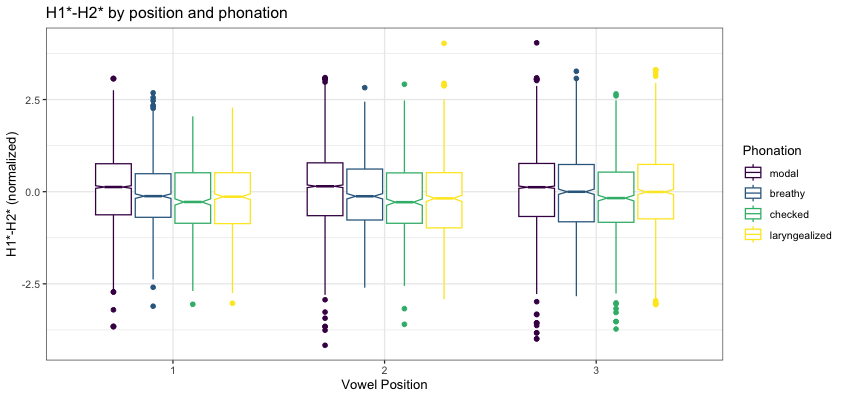
\includegraphics[width = \linewidth]{Images/h1h2_boxplot.png}
  \caption{In a notched box plot, the notches extend 1.58*IQR/sqrt(n). This gives a roughly 95\% confidence interval for comparing medians.}
  \label{fig:H1H2_box}
\end{figure}

This is further supported when we compare the plots of each of the voice qualities in a line plot using a loess smooth, as in Figure~\ref*{fig:H1H2_line}. In this plot, each of the voice qualities is plotted at each of the ten intervals of the vowel. A loess smooth was plotted over each to show how the acousitc measure functions across the ten intervals. We see that breathy, checked, and rearticulated all have a lower value than the modal at each of the first nine intervals. In the final interval, breathy and rearticulated are essentially equal to modal's value. In contrast, checked's value remains lower than the modal's value throughout the entire vowel. 

\begin{figure}[htbp]
  \centering
  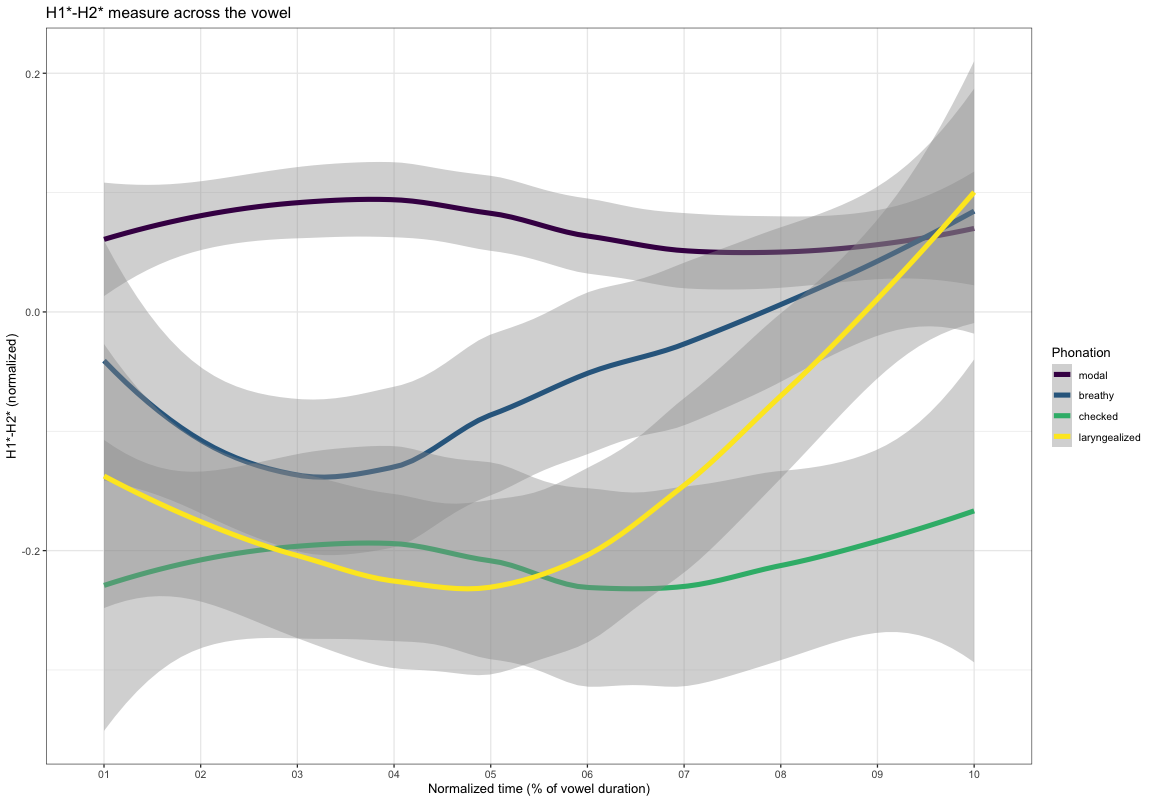
\includegraphics[width = \linewidth]{Images/h1h2_line.png}
  \caption{<caption>}
  \label{fig:H1H2_line}
\end{figure}


\begin{table}[!h]
  \centering
  \caption{Results of the linear mixed-effects model for z-scored H1*-H2*.}
  \label{tab:H1H2Results}
  \begin{tabular}{lrrrrrl}
    \lsptoprule
      & Estimate & Std. Error & df & t value & Pr(>|t|) & \\ \hline
    \textit{(Intercept)} & 0.02876 & 0.09336 & 6.17877 & 0.30809 & 0.76814 & \\
    Breathy & -0.03569 & 0.04210 & 9749.84999 & -0.84781 & 0.39656 & \\
    Checked & -0.14120 & 0.04050 & 14402.97700 & -3.48623 & \textless 0.001 & ***\\
    Rearticulated & -0.13719 & 0.04964 & 5353.41205 & -2.76340 & 0.00574 & **\\
    Position 2 & 0.00475 & 0.01339 & 19027.80227 & 0.35456 & 0.72293 & \\
    Position 3 & -0.01795 & 0.01259 & 19039.57085 & -1.42613 & 0.15385 & \\
    Tone H & 0.01597 & 0.04454 & 4340.72994 & 0.35855 & 0.71995 & \\
    Tone L & -0.07794 & 0.03218 & 8176.59285 & -2.42248 & 0.01544 & *\\
    Tone M & -0.10568 & 0.04397 & 7428.42296 & -2.40365 & 0.01626 & *\\
    Tone R & 0.28710 & 0.06918 & 10218.05414 & 4.15025 & \textless 0.001 & ***\\
    Breathy:Position 2 & 0.02104 & 0.03069 & 19046.99970 & 0.68566 & 0.49294 & \\
    Checked:Position 2 & -0.00034 & 0.03597 & 19063.65965 & -0.00949 & 0.99242 & \\
    Rearticulated:Position 2 & -0.06258 & 0.03226 & 19036.21224 & -1.94021 & 0.05237 & .\\
    Breathy:Position 3 & 0.16346 & 0.02900 & 19087.82852 & 5.63588 & \textless 0.001 & ***\\
    Checked:Position 3 & 0.04822 & 0.03400 & 19096.31688 & 1.41845 & 0.15608 & \\
    Rearticulated:Position 3 & 0.14092 & 0.03025 & 19072.44284 & 4.65848 & \textless 0.001  & ***\\
    \lspbottomrule
  \end{tabular}
\end{table}

% ------------------------------------
\subsection{H1*-A3} \label{sec:H1A3}
% ------------------------------------

\begin{figure}[htbp]
  \centering
  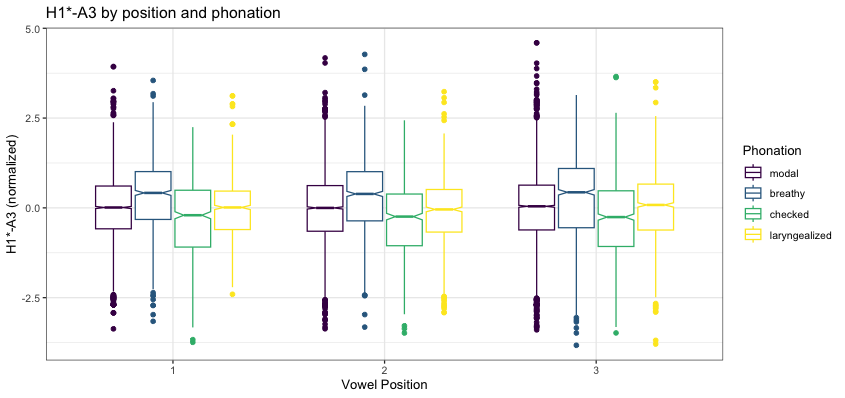
\includegraphics[width = \linewidth]{Images/h1a3_boxplot.png}
  \caption{<caption>}
  \label{fig:H1A3_box}
\end{figure}

\begin{figure}[htbp]
  \centering
  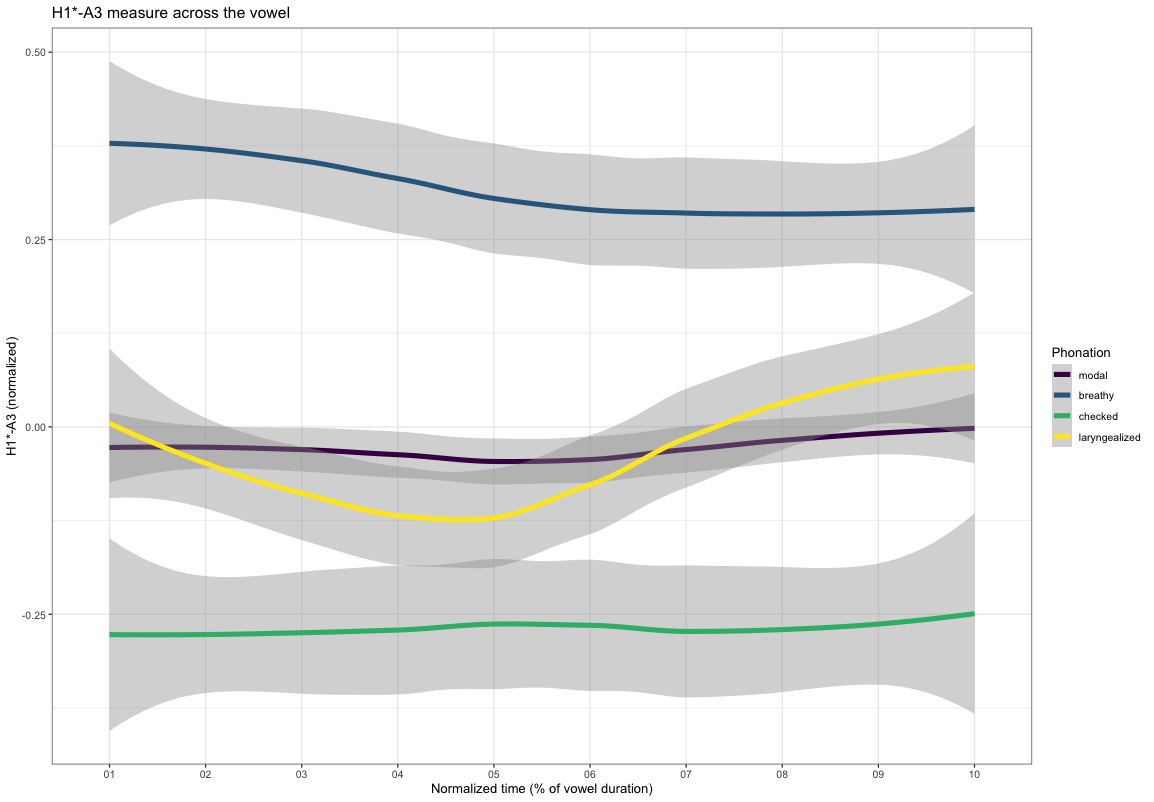
\includegraphics[width = \linewidth]{Images/h1a3_line.png}
  \caption{<caption>}
  \label{fig:H1A3_line}
\end{figure}

\begin{table}[!h]
  \centering
  \caption{Results of the linear mixed-effects model for z-scored H1*-A3.}
  \label{tab:H1A3Results}
  \begin{tabular}{lrrrrrl}
    \lsptoprule
     & Estimate & Std. Error & df & t value & Pr(>|t|) & \\ \hline
     \textit{(Intercept)} & -0.31027 & 0.07720 & 6.62348 & -4.01891 & 0.00568 & **\\
    Breathy & 0.38600 & 0.03945 & 9730.33732 & 9.78394 & \textless 0.001 & ***\\
    Checked & -0.54747 & 0.03689 & 11945.83254 & -14.84188 & \textless 0.001 & ***\\
    Rearticulated & -0.09924 & 0.04880 & 5860.06520 & -2.03384 & 0.04201 & *\\
    Position 2 & -0.01965 & 0.01153 & 19006.00934 & -1.70359 & 0.08847 & .\\
    Position 3 & 0.00304 & 0.01085 & 19013.63370 & 0.28054 & 0.77907 & \\
    Tone H & 0.26138 & 0.04422 & 4799.12698 & 5.91144 & \textless 0.001 & ***\\
    Tone L & 0.35203 & 0.03053 & 10954.20080 & 11.53172 & \textless 0.001 & ***\\
    Tone M & 0.08136 & 0.04209 & 9223.72777 & 1.93308 & 0.05326 & .\\
    Tone R & 0.73152 & 0.06454 & 14312.23532 & 11.33400 & \textless 0.001 & ***\\
    Breathy:Position 2 & -0.01424 & 0.02644 & 19019.42711 & -0.53839 & 0.59031 & \\
    Checked:Position 2 & 0.02067 & 0.03099 & 19030.35345 & 0.66688 & 0.50485 & \\
    Rearticulated:Position 2 & -0.04613 & 0.02779 & 19011.33138 & -1.66014 & 0.09690 & .\\
    Breathy:Position 3 & -0.07100 & 0.02499 & 19048.14423 & -2.84079 & 0.00451 & **\\
    Checked:Position 3 & -0.00026 & 0.02930 & 19051.95269 & -0.00876 & 0.99301 & \\
    Rearticulated:Position 3 & 0.09593 & 0.02607 & 19036.32796 & 3.68044 & \textless 0.001 & ***\\
    \lspbottomrule
  \end{tabular}
\end{table}

% ------------------------------------
\subsection{Residual H1*} \label{sec:ResidH1}
% ------------------------------------

\begin{figure}[htbp]
  \centering
  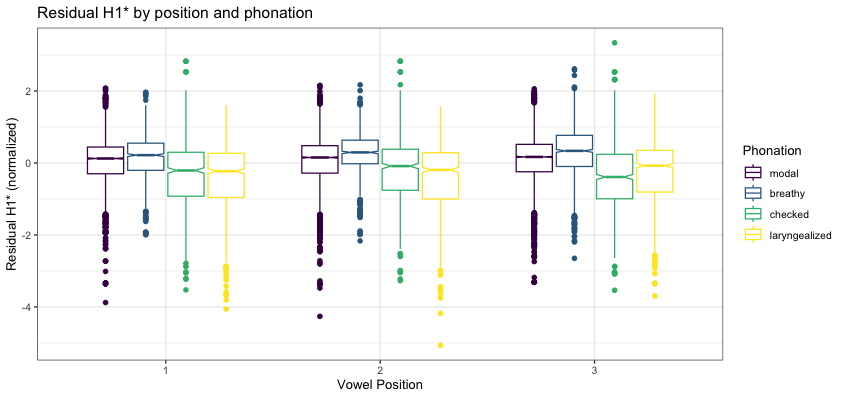
\includegraphics[width = \linewidth]{Images/residh1_boxplot.png}
  \caption{<caption>}
  \label{fig:ResidH1_box}
\end{figure}

\begin{figure}[htbp]
  \centering
  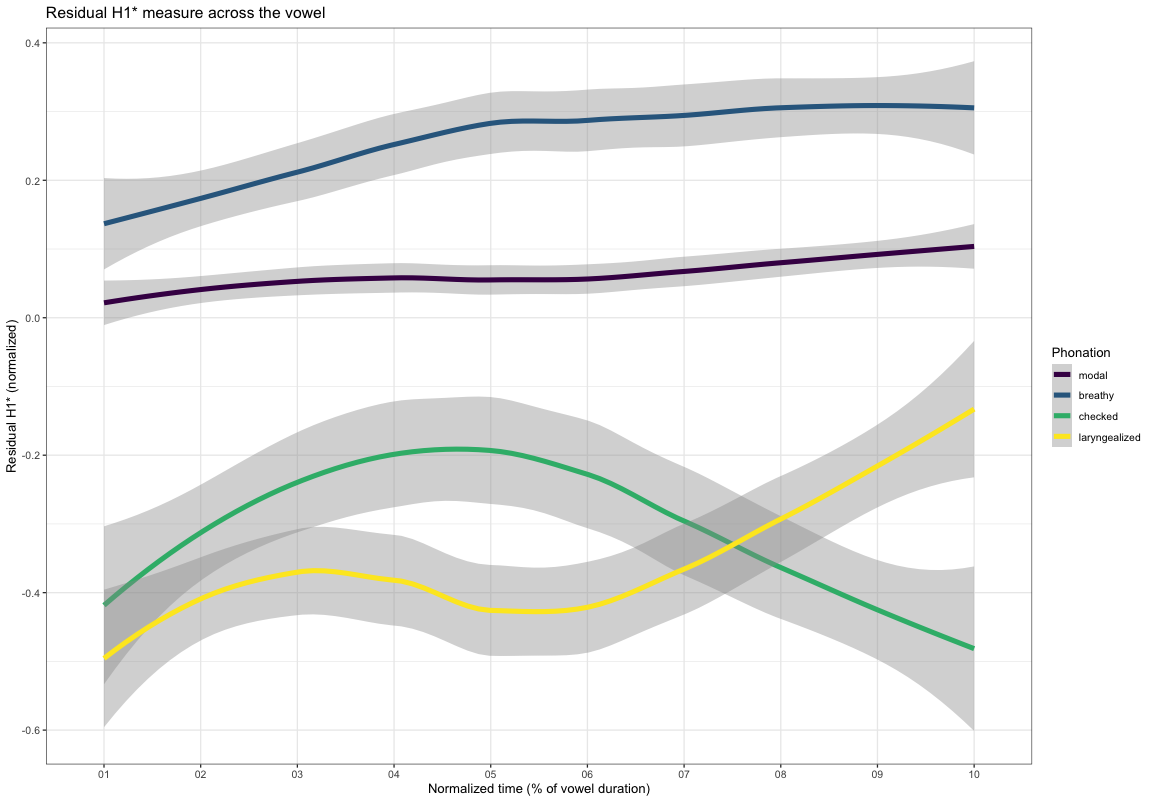
\includegraphics[width = \linewidth]{Images/residH1_line.png}
  \caption{<caption>}
  \label{fig:ResidH1_line}
\end{figure}

\begin{table}[!h]
  \centering
  \caption{Results of the linear mixed-effects model for Residual H1*.}
  \label{tab:ResH1Results}
  \begin{tabular}{lrrrrrl}
    \lsptoprule
    & Estimate & Std. Error & df & t value & Pr(>|t|) & \\ \hline 
    \textit{(Intercept)} & -0.10483 & 0.04015 & 10.71725 & -2.61084 & 0.02469 & *\\
    Breathy & 0.14997 & 0.03175 & 5393.82513 & 4.72315 & \textless 0.001 & ***\\
    Checked & -0.38554 & 0.03061 & 5905.98167 & -12.59335 & \textless 0.001 & ***\\
    Rearticulated & -0.48437 & 0.03740 & 4633.21778 & -12.95239 & \textless 0.001 & ***\\
    Position 2 & 0.01369 & 0.01027 & 19029.30204 & 1.33294 & 0.18257 & \\
    Position 3 & 0.04386 & 0.00966 & 19041.55355 & 4.54158 & \textless 0.001 & ***\\
    Tone H & 0.09272 & 0.03335 & 2975.18807 & 2.78046 & 0.00546 & **\\
    Tone L & 0.18568 & 0.02439 & 7860.40311 & 7.61295 & \textless 0.001 & ***\\
    Tone M & 0.05475 & 0.03328 & 7005.78449 & 1.64525 & 0.09996 & .\\
    Tone R & 0.33507 & 0.05257 & 9813.69066 & 6.37372 & \textless 0.001 & ***\\
    Breathy:Position 2 & 0.11599 & 0.02354 & 19049.14884 & 4.92755 & \textless 0.001 & ***\\
    Checked:Position 2 & 0.10060 & 0.02759 & 19066.47122 & 3.64602 & \textless 0.001 & ***\\
    Rearticulated:Position 2 & -0.02675 & 0.02474 & 19038.08812 & -1.08092 & 0.27975 & \\
    Breathy:Position 3 & 0.11491 & 0.02225 & 19091.32792 & 5.16510 & \textless 0.001 & ***\\
    Checked:Position 3 & -0.10327 & 0.02608 & 19100.43388 & -3.96047 & \textless 0.001 & ***\\
    Rearticulated:Position 3 & 0.12029 & 0.02320 & 19075.58487 & 5.18437 & \textless 0.001 & ***\\
    \lspbottomrule
  \end{tabular}
\end{table}

% ------------------------------------
\subsection{Model Comparison} \label{sec:Comparison}
% ------------------------------------


According to \citet{casellaStatisticalInference2002}, which is the gold standard for statistical inference in the statistics field, the best way to compare models is by comparing the AIC and the likelihood ratio between the models.
Using std error to compare models is prone to p-hacking and is heavily frowned upon by statisticians 
This was done by using the function lrtest() from the lmtest package and using the function AIC() from the base stat package
The model with the highest Log-Likelihood ratio and lowest AIC is the most robust. 

\begin{table}[!h]
  \centering
  \caption{Model comparison between H1*–H2* and Residual H1* in distinguishing SLZ phonation types.}
  \label{tab:CGComparison}
  \begin{tabular}{lllllll}
    \lsptoprule
    Phonation contrast                      & Model       & \textit{β} & Standard error & \textit{t}-value & \textit{p}      &     \\
    \hline
    \multirow[t]{3}{*}{Breathy vs Modal}       & Η1*-Η2* model & -0.03569    & 0.04210         & -0.84781  & 0.39656          &     \\
    %  & H1*-A3 model   & 0.38600  & 0.03945 & 9.78394   & \textless 0.001 & *** \\
    & Res. H1* model & 0.14997  & 0.03175 & 4.72315   & \textless 0.001   & *** \\
    \multirow[t]{3}{*}{Checked vs Modal}       & Η1*-Η2* model & -0.14120    & 0.04050         & -3.48623  & \textless 0.001 & *** \\
    %  & H1*-A3 model   & -0.54747 & 0.03689 & -14.84188 & \textless 0.001 & *** \\
    & Res. H1* model & -0.38554 & 0.03061 & -12.59335 & \textless 0.001 & *** \\
    \multirow[t]{3}{*}{Rearticulated vs Modal} & Η1*-Η2 model & -0.13719   & 0.04964         & -2.76340 & 0.00574           & **  \\
    %  & H1*-A3 model   & -0.09924 & 0.04880 & -2.03384  & 0.04201          & *   \\
    & Res. H1* model & -0.48437 & 0.03740 & -12.95239 & \textless 0.001 & *** \\
    \lspbottomrule
  \end{tabular}
\end{table}

% Please add the following required packages to your document preamble:
% \usepackage{multirow}
% \begin{table}[!h]
%   \centering
%   \caption{Model comparison between H1*–H2*, H1*-A3, and Residual H1* in distinguishing SLZ phonation types.}
%   \label{tab:CGComparison}
%   \begin{tabular}{lllllll}
%     \lsptoprule
%   Phonation contrast                      & Model       & \textit{β} & Standard error & \textit{t}-value & \textit{p}      &     \\
%   \hline
%   \multirow[t]{3}{*}{Breathy vs Modal}       & Η1*-Η2* model & -0.0345    & 0.0421         & -0.818  & 0.4135          &     \\
%   %  & H1*-A3 model   & 0.3870  & 0.0395 & 9.795   & \textless 0.001 & *** \\
%    & Res. H1* model & 0.1502  & 0.0318 & 4.716   & \textless 0.001   & *** \\
%   \multirow[t]{3}{*}{Checked vs Modal}       & Η1*-Η2* model & -0.1402    & 0.0406         & -3.457  & \textless 0.001 & *** \\
%   %  & H1*-A3 model   & -0.5464 & 0.0369 & -14.790 & \textless 0.001 & *** \\
%    & Res. H1* model & -0.3848 & 0.0307 & -12.535 & \textless 0.001 & *** \\
%   \multirow[t]{3}{*}{Rearticulated vs Modal} & Η1*-Η2 model & -0.1361    & 0.0497         & -2.740  & 0.006           & **  \\
%   %  & H1*-A3 model   & -0.0988 & 0.0487 & -2.022  & 0.0431          & *   \\
%    & Res. H1* model & -0.4856 & 0.0375 & -12.960 & \textless 0.001 & *** \\
%    \lspbottomrule
%   \end{tabular}
%   \end{table}

\begin{table}[!h]
  \centering
  \caption{LRT and AIC for the H1*-H2* and residual H1* models.}
  \label{tab:Comparison}
  \begin{tabular}{llll}
    \lsptoprule
    Model & Log-Likelihood Ratio & AIC & \Delta AIC\\
    \hline
    H1*-H2* model & -21674 & 43386.99 & 11214.54 \\
    % H1*-A3 model & -19005 & 38048.27 & 5875.82 \\
    Residual H1* model & -16067 & 32172.45 & 0 \\
    \lspbottomrule
  \end{tabular}
\end{table}

% ------------------------------------
\section{Discussion} \label{sec:Discussion}
% ------------------------------------


% ------------------------------------
\section{Conclusion} \label{sec:Conclusions}
% ------------------------------------


%------------------------------------
%BIBLIOGRAPHY
%------------------------------------

%\singlespacing
%\nocite{*}
\printbibliography[heading=bibintoc]

%-------------------------------------
\section*{Appendix 1: Elicitation word list}
%-------------------------------------

\end{document}